%===================================================================================
% Chapter: Introduction
%===================================================================================
\chapter*{Introducción}\label{chapter:introduction}
\addcontentsline{toc}{chapter}{Introducción}
%===================================================================================

\qquad 


Las técnicas de monitorización acústica automatizada se han 
convertido en una herramienta esencial para el estudio de 
comunidades de animales en su medio natural. En particular, el 
análisis del canto de los anuros ofrece información valiosa 
sobre sus estrategias de apareamiento, la dinámica de sus 
poblaciones y la salud de los ecosistemas en los que habitan \cite{blumstein2011acoustic}. 
La rana cubana \emph{Eleutherodactylus eileenae} (Dunn, 1929), 
endémica de Cuba, constituye un modelo idóneo para investigar 
estos procesos, pues sus machos forman coros nocturnos cuyos 
patrones de interacción pueden reflejar aspectos tanto 
ecológicos como de comportamiento social \cite{alonso2001patrones}.


\emph{E. eileenae}, conocido comúnmente como “Colín”, es una especie perteneciente 
a la familia \emph{Eleutherodactylidae}. Su distribución abarca desde la península 
de Guanahacabibes, en Pinar del Río, hasta la Sierra de Najasa, en Camagüey, ocupando 
diversos hábitats como bosques semideciduos, pinares y cafetales, hasta altitudes de 
aproximadamente 900 metros sobre el nivel del mar \cite{alonso2001patrones,schwartz1958new,estrada1994herpetofauna}. Durante 
el día, estos anuros se refugian en oquedades de rocas, troncos, hojarasca y 
bromelias; al anochecer, los machos ascienden a ramas y hojas, hasta alturas de 3 
metros, para emitir sus vocalizaciones.

El canto característico de \emph{E.\,eileenae} consta de dos notas diferenciadas: 
una primera “Co”, breve y de frecuencia menor, seguida de una segunda “Lin”, más 
prolongada y de frecuencia ligeramente superior. Esta estructura ha motivado el uso 
del término “Colín” para referirse tanto a cada canto individual como, 
coloquialmente, a la especie misma. Estas llamadas desempeñan un papel crucial en la 
comunicación intraespecífica, mediando aspectos relacionados con el estado 
fisiológico y la competencia territorial \cite{alonso2001patrones}. Además, se ha observado que los machos 
forman agrupaciones o “coros”, sincronizando sus cantos para aumentar la eficacia en 
la atracción de hembras y reducir el riesgo de depredación.

La presente investigación desarrolla un flujo computacional automatizado para 
procesar grabaciones de los cantos de los Colines y, a partir de él, comenzar a analizar 
 las interacciones acústicas asociadas a estos coros. 
El objetivo es comprender las 
estrategias de comunicación que emplea \emph{E.\,eileenae} en su entorno natural.
En la Figura \ref{fig:colin} se muestra un ejemplar de esta especie, y en la
Guía sonora de los anfibios de Cuba 
\footnote{Grabación disponible en: \url{https://www.fonozoo.com/fnz_detalles_registro_amphibia.php?id=97953&tipo_registro=1}}
se puede encontrar una breve grabación de su canto y otros datos relevantes.\\

\begin{figure}[h!]
    \centering
    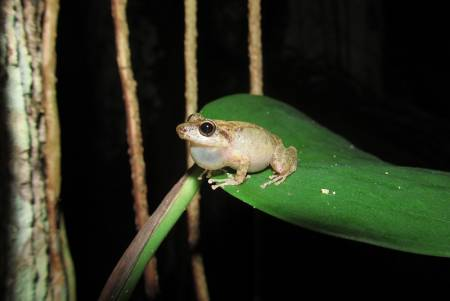
\includegraphics[width=\columnwidth]{Graphics/colin.jpg}
    \caption{Ejemplar de \emph{Eleutherodactylus eileenae}.}
    \label{fig:colin}
\end{figure}


\section{Motivación y justificación}
\label{sec:motivacion_justificacion}

La ecoacústica ha evolucionado desde la grabación pasiva hasta flujos computacionales 
que automatizan la detección de llamadas en ambientes ruidosos 
\cite{acevedo2009automated,blumstein2011acoustic}. Sin embargo, 
como resultado de la revisión bibliográfica realizada, no se conocen
estudios en Cuba que   
hayan integrado estas técnicas con modelos de interacción y causalidad.

El análisis manual de grabaciones de campo resulta lento, 
costoso y propenso a errores humanos, lo que limita la escala y 
reproducibilidad de los estudios bioacústicos. En trabajos 
previos sobre \emph{E.\,eileenae}, los investigadores 
describieron manualmente las etapas de vocalización y 
realizaron muestreos puntuales de la actividad acústica y 
trófica de los machos en la Sierra del Rosario \cite{alonso2001patrones}. 
Sin embargo, no se abordó la sincronización automática de 
múltiples micrófonos ni la clasificación sistemática de cada 
llamado, pasos indispensables para escalar el análisis a largas 
series temporales y diferentes localidades.

Además, los coros de machos implican interacciones acústicas 
cuya dinámica no se comprende completamente: ¿cómo influyen la 
densidad de individuos, la configuración espacial de los 
micrófonos y el ruido ambiental en la estructura del coro? 
¿Qué reglas simples de interacción subyacen en la sincronización 
de los “Colines”? En este contexto, un enfoque computacional reproducible
y basado en algoritmos heurísticos permitiría procesar de 
manera eficiente decenas de horas de grabaciones, discriminando 
eventos de interés (cantos de Colines) de otros sonidos 
(otra fauna, viento, tráfico) y garantizando resultados 
comparables entre campañas de muestreo.

Los resultados de la presente tesis constituyen un primer paso hacia 
el desarrollo de un 
flujo completo que abarque, desde la adquisición y sincronización 
de señales, hasta la clasificación automática de cantos y el 
modelado de interacciones acústicas, a fin de superar las 
limitaciones de los métodos manuales y aportar herramientas 
robustas para la ecoacústica de anfibios en Cuba y regiones 
semejantes.

\section{Formulación del problema}
\label{sec:formulacion_problema}

El presente trabajo se ocupa del procesamiento automático de un 
conjunto de grabaciones registradas en la Reserva de 
la Biosfera “Sierra del Rosario” con el objetivo de 
caracterizar los cantos de machos de 
\emph{Eleutherodactylus eileenae} y reconstruir la dinámica de 
sus coros. Estas grabaciones, realizadas con nueve micrófonos 
omnidireccionales dispuestos en un área de aproximadamente 20 m 
de radio, abarcan ciclos de 58 minutos de registro seguidos de 
2 minutos de descarga, durante tres noches consecutivas entre 
las 18:00 y las 06:00 horas. El entorno de captura se ve 
afectado por ruido de lluvia, viento, tráfico y la superposición 
de cantos de varios individuos, lo que plantea retos importantes 
tanto en la sincronización de señales como en la discriminación 
de los eventos acústicos relevantes frente a emisiones no 
deseadas. En la Figura \ref{fig:map} se muestra la distribución geográfica de los micrófonos en el área de estudio.

\begin{figure}[h!]
    \centering
    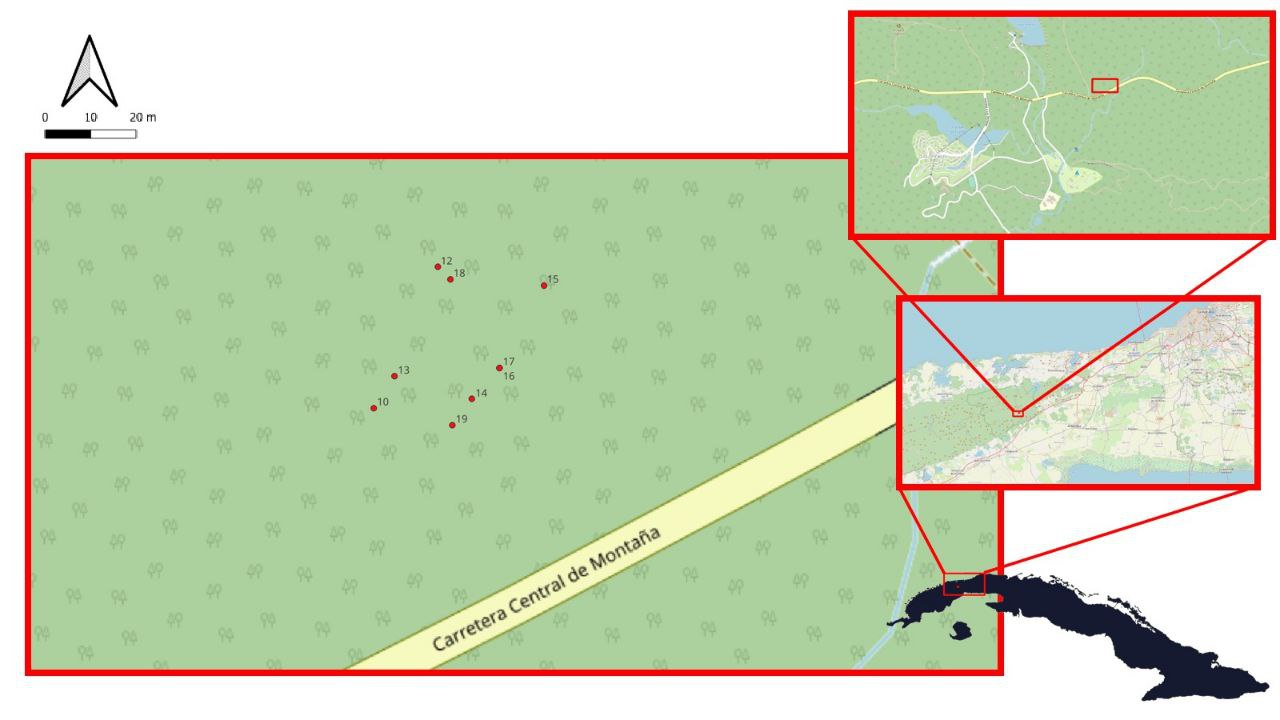
\includegraphics[width=\columnwidth]{Graphics/mic_map.jpg}
    \caption{Distribución Geográfica de los Micrófonos.}
    \label{fig:map}
\end{figure}

En este ámbito, el problema central consiste en el diseño de 
un flujo heurístico 
capaz de sincronizar con precisión las nueve pistas de audio, 
detectar de manera fiable los instantes de emisión de cada 
canto (“Colín”) y asignar cada evento al micrófono (y por tanto 
al individuo) correspondiente; a partir de ello, se extraen 
parámetros temporales y espectrales de cada llamado para 
generar un registro estructurado que sirve de base a la 
inferencia de una red de interacción inspirada en el modelo de 
Ising \cite{ising1925beitrag}. Se espera que la sincronización 
automática alcance una resolución temporal tal que permita 
distinguir llamadas superpuestas de machos vecinos, y que la 
combinación de criterios de proximidad y similitud espectral 
garantice una alta exactitud en la etiqueta de cada canto, 
validada mediante muestreo manual. Finalmente, las secuencias 
temporales resultantes se emplean para estimar los parámetros 
de interacción \(J_{ij}\), de modo que el modelo reproduzca 
con fidelidad las correlaciones de co-emisión observadas en el 
coro.  


La complejidad del problema reside en la superposición de 
señales y en la variabilidad del nivel de ruido ambiental, lo 
cual exige emplear técnicas robustas de filtrado. 
Este trabajo opta por heurísticas 
de intensidad relativa y correlación espectral para asignar cada “Colín” al micrófono y 
al individuo correspondiente, garantizando 
la reproducibilidad de los resultados y la comparabilidad con 
futuros estudios bioacústicos. Este estudio es el primero en 
Cuba en aplicar el modelo de Ising para describir 
interacciones acústicas en coros de anuros, siguiendo 
aproximaciones similares en redes 
neuronales y colonias de insectos \cite{schneidman2006weak,mora2011biological,bialek2012biophysics,reyes2019transmission,ising1925beitrag}.

\section{Hipótesis}
\label{sec:hipotesis}

Se plantea como hipótesis principal que un flujo computacional 
basado en algoritmos heurísticos para la sincronización, 
detección y clasificación de cantos de Colines podrá reproducir con un alto 
grado de fidelidad las secuencias de emisión de cada individuo 
y, a partir de ellas, inferir las interacciones acústicas 
subyacentes a la formación de coros. 


Esto fundamenta la 
viabilidad de un enfoque computacional replicable y escalable 
que, aplicado a los cantos de Colines, aporte 
nuevas perspectivas cuantitativas sobre la dinámica de los coros 
y sirva como base para futuros estudios comparativos en 
ecoacústica.  


\section{Objetivos}
\label{sec:objetivos}

El objetivo general de esta tesis es \ul{desarrollar y 
validar un flujo heurístico que, mediante la detección y 
clasificación de los cantos de \emph{E.\,eileenae}, permita 
reconstruir la dinámica de sus coros y cuantificar su 
sincronización y causalidad.}
Para ello se plantean los siguientes objetivos específicos:

\begin{enumerate}
  \item \textbf{Construir un \emph{dataset} limpio y sincronizado:}  
    \begin{itemize}
      \item Sincronizar las nueve pistas de audio utilizando referencias comunes (picos de energía) y correlación cruzada.  \cite{costa2021comparing}
      \item Eliminar ruidos de fondo (lluvia, viento, tráfico) e interferencias no deseadas.
    \end{itemize}
  \item \textbf{Detectar y asignar cada canto a su emisor:}  
    \begin{itemize}
      \item Desarrollar heurísticas de proximidad basadas en la intensidad relativa en cada micrófono.  
      \item Validar la asignación mediante muestreo manual de segmentos y cálculo de exactitud.
      \item Evaluar la consistencia de los algoritmos de detección y asignación.
      \item Comparar el rendimiento de los algoritmos diseñados.
    \end{itemize}
  \item \textbf{Inferir un modelo de interacciones acústicas:}  
    \begin{itemize}
      \item Formular la red de interacciones como un modelo de Ising con parámetros \(J_{ij}\) que cuantifiquen la co-emisión.  
      \item Estimar los \(J_{ij}\) mediante el Principio de Máxima Verosimilitud \cite{fisher1912maximum} y algoritmos de descenso por gradiente.
      \item Evaluar la idoneidad del modelo de Ising mediante una comparación con el modelo Independiente en cuanto a su capacidad para predecir los patrones de cantos.
    \end{itemize}
\end{enumerate}


\section{Propuesta de solución}
\label{sec:propuesta_solucion}

Para dar respuesta al problema planteado, se propone un 
flujo de trabajo modular que integre cuatro etapas principales: 
sincronización, filtrado, asignación de 
emisores y modelado de interacciones. En primer lugar, la 
sincronización de las nueve pistas de audio se realiza 
mediante la aplicación de correlación cruzada sobre los histogramas
de distribución de distancias temporales entre los picos de energía de los audios 
y un punto de referencia. A continuación, se 
aplica un filtro que consiste en una poda espectral
basada en el percentil 99.9 de la amplitud por frecuencia.
Con ello se busca atenuar 
ruido de baja (viento, tráfico) y alta frecuencia (insectos).  

En la tercera fase se asigna cada 
llamado al micrófono más adecuado mediante heurísticas de 
intensidad relativa. 
Finalmente, la información temporal y espectral extraída de cada 
evento sirve para construir un grafo de interacciones, 
modelado con un enfoque de máxima verosimilitud en un sistema 
análogo al modelo de Ising. El ajuste de los 
parámetros \(J_{ij}\) se lleva a cabo mediante un algoritmo de 
descenso por gradiente.  

Este flujo, además de automatizar completamente la extracción de 
datos, permite validar la hipótesis mediante 
métricas objetivas de precisión y reproducibilidad, y ofrece 
una herramienta extensible a otros sistemas de ecoacústica con 
configuraciones similares.  


\section{Estructura del Documento}
\label{sec:estructura_documento}

Para explicar la solución propuesta y el flujo de trabajo, 
se diseñó la siguiente estructura del presente documento. 
En el Capítulo 1 se revisan los antecedentes y actualidad en cuanto a 
detección y 
clasificación de llamadas bioacústicas, con especial énfasis 
en métodos de sincronización y filtrado de señales. 
El Capítulo 2 detalla la metodología empleada: adquisición y 
preprocesamiento de las grabaciones, tanto el diseño de 
algoritmos heurísticos 
para la detección de los “Colines” como la asignación de cada 
canto a su emisor, y la formulación del modelo de interacciones 
basado en Ising con inferencia por máxima verosimilitud y 
descenso por gradiente. En el Capítulo 3 se presentan los 
resultados: evaluación de la precisión de 
sincronización, rendimiento de los detectores de canto, 
exactitud de la asignación micrófono-Colín y análisis de las 
interacciones inferidas \(\{J_{ij}\}\). Además en las 
Conclusiones se discuten las aportaciones principales, las 
implicaciones ecológicas y computacionales y las limitaciones 
del estudio.
Finalmente, en las Recomendaciones se presentarán sugerencias 
generales basadas en los resultados, destinadas a 
orientar mejoras metodológicas, proponer nuevas líneas de 
investigación y facilitar la aplicación práctica del enfoque 
desarrollado en estudios futuros.  

% -----------------------------------------------------------------------



% La rana \emph{Eleutherodactylus eileenae} (Dunn, 1929) es una especie 
% de la familia \emph{Eleutherodactylidae}, endémica de Cuba. 
% Se distribuye desde la península de Guanahacabibes, Pinar del Río, 
% hasta la Sierra de Najasa, en la provincia de Camagüey. 
% Ocupa hábitats como bosques semideciduos, pinares y cafetales
% en altitudes de hasta 900 metros sobre el nivel del mar. 
% Durante el día permanece oculta en
% oquedades de rocas y troncos, y entre la hojarasca y bromelias.
% Durante la noche los machos ascienden 
% para vocalizar en ramas y hojas de hasta 3 m de altura. \cite{alonso2001patrones}
% En la Figura \ref{fig:colin} se muestra un ejemplar de esta especie, y en la
% Guía sonora de los anfibios de Cuba 
% \footnote{Grabación disponible en: \url{https://www.fonozoo.com/fnz_detalles_registro_amphibia.php?id=97953&tipo_registro=1}}
% se puede encontrar una breve grabación de su canto y otros datos relevantes.\\

% \begin{figure}[h!]
%     \centering
%     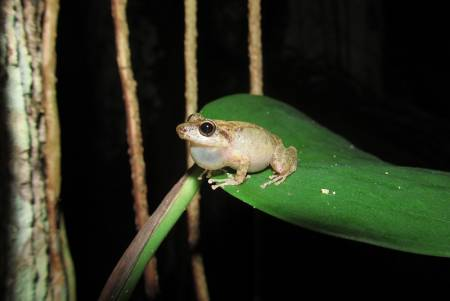
\includegraphics[width=\columnwidth]{Graphics/colin.jpg}
%     \caption{Ejemplar de \emph{Eleutherodactylus eileenae}.}
%     \label{fig:colin}
% \end{figure}


% El canto de \emph{E.\,eileenae} consta de dos notas 
% diferenciadas: una primera “Co” breve y de frecuencia menor, 
% seguida de “Lin” más prolongada y de frecuencia ligeramente 
% superior, nombradas de esta forma para imitar el sonido producido. 
% Por tal motivo y por simplicidad se procederá a nombrar “Colín” a cada uno de los cantos 
% y también se utilizará como nombre coloquial de la especie. 
% Estas llamadas median parámetros bioacústicos 
% vinculados al estado fisiológico y a la competencia territorial. 
% Además, se ha observado que los machos forman agrupaciones 
% (“coros”), sincronizando pulsos y modulaciones para incrementar 
% la eficacia de atracción de hembras y reducir el riesgo de 
% depredación. La presente investigación se centrará en el estudio de dichos
% coros y los cantos con fines de apareamiento de los Colines.



% \section{Características del \emph{dataset} de grabaciones}

% El canto de \emph{E.\,eileenae} se produce en la noche,
% cuando los machos se agrupan para vocalizar, 
% con picos de actividad en los meses calurosos y lluviosos del año y 
% en las horas de la tardenoche y la madrugada.
% Con el objetivo de adquirir datos para los estudios de la especie,
% el grupo de investigación dirigido por el Dr. Roberto Alonso, de la Facultad de Biología de la Universidad de La Habana,
% realizó un conjunto de grabaciones de campo en la zona de la 
% Reserva de la Biosfera “Sierra del Rosario”. Después de identificar ciertos
% individuos y los sitios donde usualmente se ubicaban para emitir sus cantos, se colocaron
% 9 micrófonos (cada uno aproximadamente a 1 metro de distancia de su Colín más cercano)
% cuya activación remota permitió el registro de la información acústica del coro en cuestión.
% Todos los dispositivos eran del mismo modelo, unidireccionales, y eran activados simultáneamente para comenzar a grabar
% 58 minutos consecutivos, utilizar 2 minutos para guardar los datos adquiridos y luego volver a comenzar a grabar.
% Esto se hizo durante 3 noches, en los períodos comprendidos entre las 18:00 horas y las 6:00 horas del día siguiente, entre los días
% 20 y 23 de octubre de 2023. En la Figura \ref{fig:map} se muestra la distribución geográfica de los micrófonos en el área de estudio.
% Como se puede apreciar, los micrófonos fueron colocados en un área con un radio de aproximadamente 20 metros.\\

% \begin{figure}[h!]
%     \centering
%     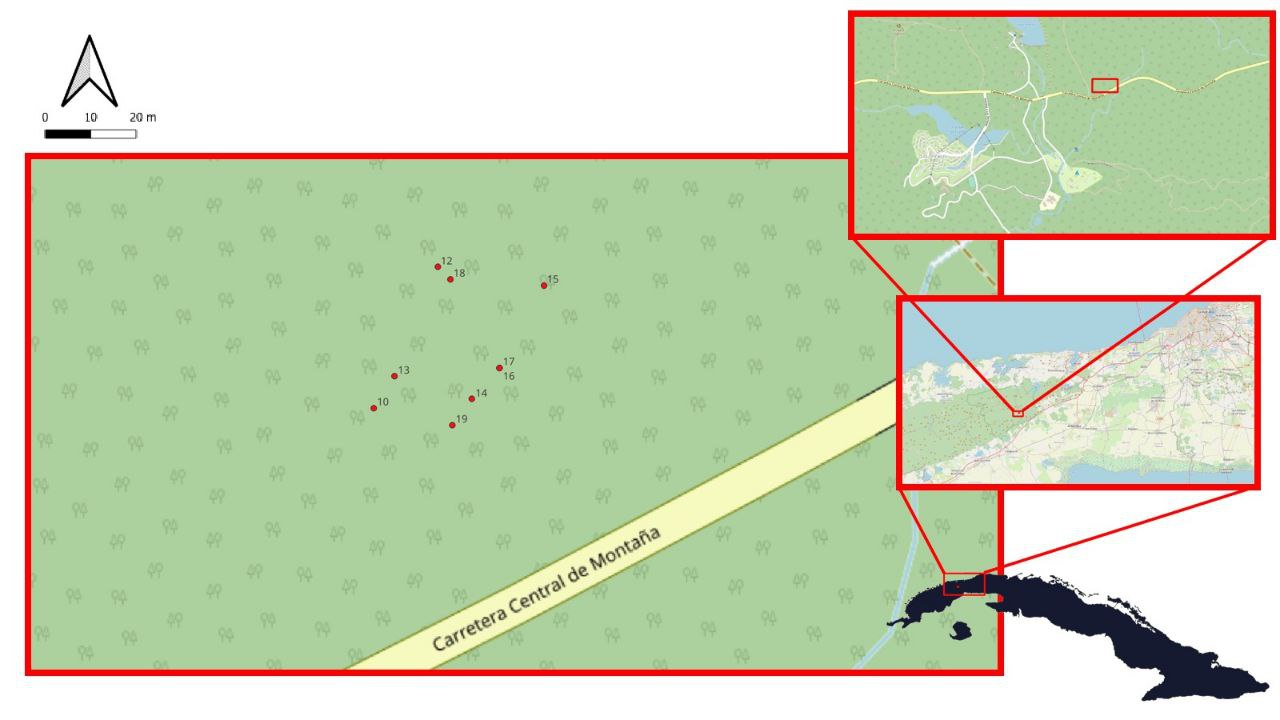
\includegraphics[width=\columnwidth]{Graphics/mic_map.jpg}
%     \caption{Distribución Geográfica de los Micrófonos.}
%     \label{fig:map}
% \end{figure}

% Debido a que los micrófonos son omnidireccionales y están situados 
% relativamente cercanos entre sí, en cada uno se registran no solamente
% los cantos del individuo de Colín más cercano, sino también cantos de especímenes
% cercanos, sonidos del ambiente natural de la zona, e incluso ruidos de 
% agentes artificales como autos pasando por una carretera cercana.



% \section{Motivaciones de la investigación}

% Como parte de los estudios sobre la ecología de esta especie de anuros
% se quiere profundizar en lo que se conoce sobre las características de sus cantos,
% de sus métodos de comunicación y su comportamiento social. Además se quiere 
% saber si realmente se organizan en coros, y si ese fuera el caso, analizar la
% estructura de dichos coros, la posible existencia de un líder o protagonista,
% o de manera general estudiar las interacciones en el sistema formado por los Colines
% machos mientras cantan para atraer a las hembras.\\

% Hasta el momento, el trabajo para procesar los audios recopilados se realizaba de forma manual
% con \emph{softwares} no automáticos. La identificación manual de cada llamado (etiquetado por 
% individuo, hora y localización) resulta extremadamente lenta, 
% sujeta a errores humanos y poco reproducible. Dichas razones,
% sumadas a la búsqueda de avances más eficientes y rigurosos, motivaron el tratamiento
% del problema desde un enfoque computacional, para automatizar los procesos
% y poder modelar matemáticamente el sistema de interacción entre los Colines.\\ 


% \section{Problema científico}

% El problema planteado consiste en, dado un \emph{dataset} de grabaciones
% de campo de un coro de Colines hechas con 9 micrófonos omnidireccionales,
% procesar los datos para obtener la información de los cantos de cada uno de 
% los individuos implicados (momento del canto, frecuencia, energía) para
% analizar la estructura de dicho coro. \\

% Que los dispositivos de sean omnidireccionales plantea la dificultad de
% que en una misma grabación se registra la información de sonidos que no interesan,
% como otros animales, autos e incluso Colines que no son los más cercanos al aparato.
% Por lo tranto surge la necesidad de diseñar un proceso para discriminar correctamente
% estos datos, y obtener una asigación Micrófono-Colín. Además es evidente que se impone
% encontrar una forma de eliminar el ruido y “limpiar” los audios. 
% También se debe verificar la correcta sincronización de las grabaciones,
% pues a pesar de la activación remota y simultánea, el posible error de \emph{hardware}
% podría comprometer la precisión de los resultados.\\

% Convendría modelar matemáticamente el sistema
% para cuantificar las interacciones entre los especímenes y llevar a cabo un estudio
% de causalidad. Para ello se propone la utilización de un recurso clásico
% de la Física Estadística, el Modelo de Ising. \cite{chau2017inverse}

% \section{Objetivos de la tesis}

% El objetivo principal de esta tesis es diseñar, implementar y validar un flujo computacional automatizado para la detección, clasificación y análisis de los cantos de apareamiento de \emph{Eleutherodactylus eileenae}, con el fin de reconstruir la estructura de sus coros y modelar las interacciones acústicas entre individuos mediante el enfoque del modelo de Ising.
% Para ello se plantean los siguientes objetivos específicos:

% \begin{enumerate}
%   \item Construir un \emph{dataset} limpio de grabaciones que permita extraer estadísticas fiables y facilitar la interpretación de resultados.
%   \item Desarrollar un método de sincronización automática de las señales grabadas por los nueve micrófonos para asegurar la consistencia temporal del \emph{dataset}.
%   \item Implementar técnicas de eliminación de ruido de fondo y filtrado de eventos no deseados (otros animales, vehículos, artefactos ambientales).
%   \item Diseñar y comparar algoritmos para la obtención de las secuencias de cantos de cada Colín.
%   \item Validar la consistencia, precisión y reproducibilidad de los métodos propuestos.
%   \item Modelar matemáticamente la red de interacciones acústicas entre individuos utilizando el modelo de Ising:
%     \begin{itemize}
%       \item Formulación del problema como Principio de Máxima Verosimilitud.
%       \item Implementación de algoritmos de Descenso por Gradiente para la inferencia de los parámetros \(J_{ij}\) (interacción entre el individuo $i$ y $j$).
%     \end{itemize}
%   \item Analizar la idoneidad del modelo de Ising para describir la causalidad en los coros, comparando las interacciones inferidas con comportamientos observados.
%   \item Interpretar los resultados y extraer conclusiones ecológicas y computacionales que permitan proponer recomendaciones para estudios bioacústicos futuros.
% \end{enumerate}

% Para abordar estos objetivos, la tesis se organiza en los siguientes capítulos:
% \begin{description}
%   \item[Capítulo 1:] \emph{Detección de individuos a partir de señales de audio}. Revisión del estado del arte en detección y clasificación de llamadas bioacústicas.
%   \item[Capítulo 2:] \emph{Métodos y metodologías}. Representación de audio como \emph{mel}-espectrogramas, sincronización, eliminación de ruido, diseño de algoritmos de identificación y discriminación de Colines, y formulación del modelo de Ising con su inferencia mediante máxima verosimilitud y descenso por gradiente.
%   \item[Capítulo 3:] \emph{Resultados e interpretación}. Evaluación de la sincronización automática, obtención de secuencias de cantos, hipótesis de comportamiento espectral, comparación de algoritmos, pruebas de consistencia y precisión, y análisis de las interacciones inferidas \(\{J_{ij}\}\) en el modelo de Ising.
%   \item[Conclusiones y Recomendaciones:] Síntesis de hallazgos, discusión de implicaciones ecológicas y computacionales, limitaciones del estudio y propuestas de trabajo futuro.
% \end{description}





% % \section*{Contexto histórico y social}
% % En las últimas décadas, el análisis automatizado de datos biológicos ha revolucionado campos tan diversos como la ecoacústica y los estudios de comportamiento colectivo. En particular, los avances en aprendizaje automático han permitido procesar grandes volúmenes de grabaciones de campo para monitorear especies silvestres de manera más precisa y reproducible :contentReference[oaicite:0]{index=0}. Paralelamente, la Física Estadística ha contribuido al entendimiento de sistemas complejos mediante modelos de interacción par a par, como el modelo de Ising, aplicado originariamente a redes de espines y recientemente extendido a inferencia de redes biológicas :contentReference[oaicite:1]{index=1}.  

% % \section*{Antecedentes del problema científico}
% % En Cuba, los estudios sobre comportamiento colectivo se han centrado tradicionalmente en sistemas como colonias de hormigas, demostrando cómo interacciones locales generan patrones globales de organización sin control centralizado :contentReference[oaicite:2]{index=2}. En el ámbito de los anfibios, la comunicación acústica ha servido como modelo para entender la señalización social y la toma de decisiones del sistema nervioso :contentReference[oaicite:3]{index=3}. Sin embargo, la mayoría de los análisis de cantos de ranas se realiza aún de forma manual, lo que limita la escala y reproducibilidad de los estudios :contentReference[oaicite:4]{index=4}.

% % \section*{Breve presentación de la problemática}
% % La rana cubana \emph{Eleutherodactylus eileenae} (Dunn, 1929) es un anuro endémico que forma coros de machos durante la noche para atraer hembras. Cada canto, denominado “Colín”, consta de dos notas diferenciadas (“Co” y “Lin”) que varían en frecuencia y duración :contentReference[oaicite:5]{index=5}. Para estudiar la estructura de estos coros y las interacciones acústicas entre individuos, se dispusieron redes de micrófonos que registraron cientos de horas de audio en ambientes ruidosos, lo que plantea retos de sincronización, filtrado de ruido y asignación automática de cada evento acústico a su emisor :contentReference[oaicite:6]{index=6}.

% % \section*{Actualidad y novedad científica}
% % Hoy día, la integración de sensores pasivos con algoritmos de inteligencia artificial permite extraer patrones bioacústicos a escala inédita :contentReference[oaicite:7]{index=7}. No obstante, aplicar modelos de inferencia estadística, como el modelo de Ising, para cuantificar las interacciones en un coro de ranas nocturnas constituye una aproximación novedosa que une ecoacústica, teoría de redes y computación biomédica.  

% % \section*{Importancia teórica y práctica}
% % Teóricamente, el estudio contribuirá a validar el modelo de Ising en sistemas biológicos reales, más allá de ensayos in silico :contentReference[oaicite:8]{index=8}. Prácticamente, facilitará protocolos automáticos de monitoreo de poblaciones de anfibios, mejorando la eficiencia de la conservación y el control de indicadores ecológicos en zonas protegidas.  

% % \section*{Diseño teórico}
% % \subsection*{Problema científico}
% % Dado un \emph{dataset} de grabaciones de un coro de \emph{E.\,eileenae} obtenidas con nueve micrófonos omnidireccionales, se busca procesar las señales para extraer los instantes, frecuencias y energías de cada canto y reconstruir la red de interacciones acústicas entre individuos.  

% % \subsection*{Objeto de estudio}
% % Las interacciones de fase y coincidencia temporal de los cantos de machos de \emph{E.\,eileenae} en un área de estudio en la Reserva de la Biosfera “Sierra del Rosario”, Cuba.  

% % \subsection*{Objetivos}
% % \begin{itemize}
% %   \item \textbf{General:} Diseñar y validar un flujo computacional para la detección, clasificación y modelado de interacciones acústicas en coros de \emph{E.\,eileenae} mediante el modelo de Ising.
% %   \item \textbf{Específicos:}
% %     \begin{enumerate}
% %       \item Construir un \emph{dataset} limpio y sincronizado de grabaciones nocturnas.
% %       \item Implementar filtrado de ruido y asignación automática de eventos a individuos.
% %       \item Desarrollar y comparar algoritmos de detección basada en \emph{mel}-espectrogramas y aprendizaje supervisado.
% %       \item Inferir los parámetros de interacción \(\{J_{ij}\}\) usando máxima verosimilitud y descenso por gradiente.
% %       \item Evaluar la consistencia y precisión de los métodos propuestos.
% %     \end{enumerate}
% % \end{itemize}

% % \subsection*{Campo de acción}
% % Bioacústica, procesamiento de señales, aprendizaje automático, teoría de redes y Física Estadística aplicada a ecología.  

% % \subsection*{Hipótesis científica}
% % El modelo de Ising, inferido sobre un \emph{dataset} sincronizado y filtrado de cantos de \emph{E.\,eileenae}, reproducirá fielmente las interacciones acústicas observadas y permitirá distinguir mecanismos de sincronización en el coro.

% % \section*{Estructuración del trabajo}
% % \begin{description}
% %   \item[Capítulo 1:] Estado del arte en detección y clasificación de llamadas bioacústicas.
% %   \item[Capítulo 2:] Metodologías: adquisición y limpieza de datos, sincronización, algoritmos de detección y filtrado, formulación del modelo de Ising e inferencia de parámetros.
% %   \item[Capítulo 3:] Resultados: evaluación de sincronización, obtención de secuencias de cantos, comparación de métodos, análisis de interacciones \((J_{ij})\) e idoneidad del modelo.
% %   \item[Capítulo 4:] Conclusiones y recomendaciones: implicaciones ecológicas, limitaciones, aportes computacionales y líneas futuras.
% % \end{description}


























